\documentclass[12pt,letterpaper]{article}
\usepackage{graphicx,float}
\usepackage{hyperref}
\usepackage{amsmath,amsfonts,amssymb}
\usepackage{tikz}
\usetikzlibrary{arrows.meta,calc}


\setlength{\textwidth}{6.5in}
\setlength{\oddsidemargin}{0in}
\setlength{\textheight}{9in}
\setlength{\topmargin}{-.25in}
%DEFINE THEREFORE FUNCTION
\def\therefore{\boldsymbol{\text{ }
\leavevmode
\lower0.4ex\hbox{$\cdot$}
\kern-.5em\raise0.7ex\hbox{$\cdot$}
\kern-0.55em\lower0.4ex\hbox{$\cdot$}
\thinspace\text{ }}}

\title{Draft Report}
\author{Warvin Hassan}

\begin{document}
\maketitle
\pagebreak
\tableofcontents
\pagebreak
\part{Introduction}
The Total Graph Value (TGV) of a graph is the sum of the products of edge weights across all spanning trees of the graph. To determine the TGV for a weighted graph, all spanning trees of the graph must first be identified. A spanning tree is a subgraph that includes all the vertices of the original graph, is connected, and contains no cycles. For each spanning tree, the product of the weights of its edges is calculated. The TGV is then obtained by summing these products over all spanning trees. This value provides insight into the relationship between the graph's structure and its edge weights. In this report, we focus on calculating the TGV for various types of graphs, with an emphasis on trees, cycles, divided cycles, and complete graphs. Specifically, we investigate how the assignment of weights to edges affects the TGV and explore methods for maximizing this value. The methods used in this study are primarily computational in nature, involving the application of combinatorial principles, graph algorithms, and symbolic computation using the SageMath software environment.\\

\pagebreak
% PART 1
\part{Results}

% SECTION 1
\section{Trees}  \label{P}

We found that for trees the total graph value was rather trivial since there was only one spanning tree for any given tree and so the product of these graphs is the total graph value.

% SUBSECTION 1.1
\subsection{Code}

% FIGURE 1
	\begin{figure}[hbt!]  
		\begin{center}
		\includegraphics[width=4in]{f1.1.jpg}
		\end{center}
		\caption{\label{OrBx} Simple tree and its results using SageMath}
	\end{figure}
	

  
% SUBSECTION 1.2
\subsection{Proof}
The following proof will show that it does not matter how one assigns weights to trees by proving that the total value of the respective graph remains the same.\\

Let $n\in\mathbb{Z}^{+}$, then a tree $T_{n}$ on $n$ vertices has $n-1$ edges and is already a tree. Since the graph is a tree the only spanning tree is the tree itself, with the total graph value being the product of the weights of all the edges in the tree $$TGV=w_{1}\cdot w_{2}\cdot\ldots\cdot w_{n-1.}$$
$\blacksquare$\\

% SECTION 2
\section{Cycles} \label{C}
Cycles were also pretty trivial as we found that regardless of the way we distributed the weights on the edges we got the same total graph value and this was due to the symmetery of cyclic graphs. We noticed that the number of spanning trees of a cycle was also the same number of vertices/edges of that same cycle. This is because a spanning tree is found by removing an edge of the cycle.

% SUBSECTION 2.1
\subsection{Code}
 
% FIGURE 2
	\begin{figure}[h!]
  \begin{center}
    \includegraphics[width=4.2in]{f2.1.jpg}
    \includegraphics[width=4.2in]{f2.11.jpg}
    \caption{\label{Patch} Same Results for Two Distinctly Distributed C5s}
  \end{center}
	\end{figure}
  
% SUBSECTION 2.2
\subsection{Proof}

Let the two weighted $n$-cycles be denoted as $C_{1}$ and $C_{2}$. The Edges of $C_{1}$ can be represented as $E_{1}=\{e_{1},e_{2},\ldots,e_{n}\}$ and the edges of $C_{2}$ as $E_{2}=\{f_{1},f_{2},\ldots,f_{n}\}$. The weights assigned to the edges of both $C_{1}$ and $C_{2}$ are derived from the same set $W=\{w_{1},w_{2}\ldots,w_{n}\}$ and are assigned randomly; $i.e.,$ for some weight $w_{j}=e_{a}$ and $w_{j}=f_{b}$ where $a,b \le n$. In an \( n \)-cycle \( C_n \), a spanning tree is formed by removing exactly one edge from the cycle, leaving a connected graph with \( n-1 \) edges. Since the edges of the cycles \( C_1 \) and \( C_2 \) are in bijective correspondence through the mapping \( m \), and the weights are derived from the same set \( W \), the spanning trees of \( C_1 \) and \( C_2 \) are also in bijective correspondence.\\

For any weight assignment, the product of the weights for a given spanning tree is determined by the \( n-1 \) edges that remain. Because the mapping \( m \) ensures that the same weights correspond to edges in both cycles, the sum of the products of weights across all spanning trees (the total graph value, \( TGV \)) must be the same for \( C_1 \) and \( C_2 \).\\

Thus, the total graph values for \( C_1 \) and \( C_2 \) are equal:
\[
TGV(C_1) = TGV(C_2).
\]$\blacksquare$\\

% SECTION 3
\section{Divided Cycles} \label{DC}
We found that divided cycles behaved rather predictibly since they were essentially cycles with an extra edge. The extra edge seemed to contribute insignificantly to the total overall graph value because it simply was not included in many spanning trees. With that being said, we noticed that while assigning the lowest weight to the dividing edge did indirectly contribute to the total graph value, that alone is not enough to determine the max value for any given divided cycle. Other factors, such as the distribution of weights along the cycle edges, played a significant role in determining the total graph value. Specifically, configurations that balanced the weights across the cycle edges while minimizing the impact of the dividing edge on critical spanning tree combinations tended to yield higher graph values. This suggests that the interplay between the edge weights and the structural redundancy of spanning trees in divided cycles must be carefully considered to optimize the total graph value, rather than relying solely on minimizing the weight of the dividing edge.

% SUBSECTION 3.1
\subsection{Code}

% FIGURE 3
	\begin{figure}[h!]  
    \begin{center}
    \includegraphics[width=5in]{f3.1.jpg}
    \caption{\label{Marble} The Maximum value for a $C_6 + 1$.}
    \end{center}
	\end{figure}

% FIGURE 4
\begin{figure}[hbt!]  
    \begin{center}
    \includegraphics[width=5in]{f3.11.jpg}
    \caption{\label{Marble2} Many $C_6 + 1$ permutations with same max value.}
    \end{center}
	\end{figure}
\newpage
% SUBSECTION 3.2
\subsection{Proof}

Let \( C_n \) be a cycle graph with \( n \) vertices, and let the edges of \( C_n \) be labeled \( e_1, e_2, \dots, e_n \), with corresponding edge weights \( w_1, w_2, \dots, w_n \). Let \( e_d \) denote the dividing edge, which connects two non-adjacent vertices of \( C_n \) and ``divides'' the cycle. The total graph value \( T(G) \) is defined as the sum of the products of edge weights over all spanning trees of \( G \). To analyze the impact of assigning weights, we partition the spanning trees into three disjoint sets.\\

Fix an edge on the cycle $e_{j}$. The first set, \( S_1 \), consists of all spanning trees that either include both \( e_d \) and some edge \( e_j \), or exclude both \( e_d \) and \( e_j \). Notice that swapping the weights of \( e_d \) and \( e_j \) does not alter the contribution of the spanning trees in \( S_1 \), as the product terms involving \( w_d \) and \( w_j \) remain identical. \( S_2 \) is the set that includes either \( e_j \) or \( e_d \) but not both and \( S_2 \neq \emptyset \) Finally, \( S_3 \) is the converse set of \( S_2 \), $i.e.,$ the set does not take one edge from each side of the divider but those that may take two from one side. \\

Since \( w_j > w_d \) by assumption, the sign of the change depends on the difference of the spanning trees that include \( e_d \) and those that include \( e_j \). The key observation is that the contribution of spanning trees that include \( e_j \) is larger because \( e_j \) is a cycle edge, and cycle edges appear in more spanning trees compared to \( e_d \), which connects non-adjacent vertices.\\

Notice that W.L.O.G. each tree that contains $e_d$, but not $e_j$ has a TGV that corresponds to a tree that contains $e_j$ but not $e_d$ and all of the other edges remain the same. However the converse of this is not true. Refer to figures 5 and 6 to see this.\\

\begin{figure}[h!]
\centering
\begin{tikzpicture}[scale=0.6, every node/.style={circle, fill=black, inner sep=1.5pt},
                    edge/.style={thick}, arrow/.style={-{Stealth[scale=1.2]}}]

% First row
\begin{scope}[shift={(0, 0)}]
    % Graph 1
    \foreach \i in {1,...,6} {
        \node (A\i) at ({60*(\i-1)}:1) {};
    }
    \draw[edge] (A1) -- (A2);
    \draw[edge] (A2) -- (A3);
    %\draw[edge] (A3) -- (A4);
    \draw[edge] (A4) -- (A5);
    \draw[edge] (A5) -- (A6);
    %\draw[edge] (A6) -- (A1);

    \draw[edge] (A1) -- (A4); % Dividing edge
    \draw[draw=none] (0.2, 0.1) -- (0.2, 0.1) node[fill=none, midway, above left, rotate=45] {$e_{d}$};
    %\draw[draw=none] (A2) -- (A3) node[fill=none, midway, below] {$e_{j}$}; % Label for a cycle edge

    % Arrow to Graph 2
    \draw[<->, thick] (1.5, 0) -- (2.5, 0);

    % Graph 2
    \begin{scope}[shift={(4, 0)}]
        \foreach \i in {1,...,6} {
            \node (B\i) at ({60*(\i-1)}:1) {};
        }
        \draw[edge] (B1) -- (B2);
        \draw[edge] (B2) -- (B3);
        %\draw[edge] (B3) -- (B4);
        \draw[edge] (B4) -- (B5);
        \draw[edge] (B5) -- (B6);
        \draw[edge] (B6) -- (B1);
        %\draw[edge] (B1) -- (B4); % Dividing edge
        %\draw[draw=none] (0.2, 0.1) -- (0.2, 0.1) node[fill=none, midway, above left, rotate=45] {$e_{d}$}; 
        \draw[draw=none] (B6) -- (B1) node[fill=none, midway, below, rotate=45] {$e_{j}$};
    \end{scope}
\end{scope}

% Second row
\begin{scope}[shift={(0, -3)}]
    % Graph 3
    \foreach \i in {1,...,6} {
        \node (C\i) at ({60*(\i-1)}:1) {};
    }
    \draw[edge] (C1) -- (C2);
    %\draw[edge] (C2) -- (C3);
    \draw[edge] (C3) -- (C4);
    \draw[edge] (C4) -- (C5);
    \draw[edge] (C5) -- (C6);
    %\draw[edge] (C6) -- (C1);
    \draw[edge] (C1) -- (C4); % Dividing edge
    \draw[draw=none] (0.2, 0.1) -- (0.2, 0.1) node[fill=none, midway, above left, rotate=45] {$e_{d}$};
    %\draw[draw=none] (C6) -- (C1) node[fill=none, midway, below, rotate=45] {$e_{j}$};

    % Arrow to Graph 4
    \draw[<->, thick] (1.5, 0) -- (2.5, 0);

    % Graph 4
    \begin{scope}[shift={(4, 0)}]
        \foreach \i in {1,...,6} {
            \node (D\i) at ({60*(\i-1)}:1) {};
        }
        \draw[edge] (D1) -- (D2);
        %\draw[edge] (D2) -- (D3);
        \draw[edge] (D3) -- (D4);
        \draw[edge] (D4) -- (D5);
        \draw[edge] (D5) -- (D6);
        \draw[edge] (D6) -- (D1);
        %\draw[edge] (D1) -- (D4); % Dividing edge
        %\draw[draw=none] (0.2, 0.1) -- (0.2, 0.1) node[fill=none, midway, above left, rotate=45] {$e_{d}$}; 
        \draw[draw=none] (D6) -- (D1) node[fill=none, midway, below, rotate=45] {$e_{j}$};
    \end{scope}
\end{scope}

% Third row
\begin{scope}[shift={(0, -6)}]
    % Graph 5
    \foreach \i in {1,...,6} {
        \node (E\i) at ({60*(\i-1)}:1) {};
    }
    %\draw[edge] (E1) -- (E2);
    \draw[edge] (E2) -- (E3);
    \draw[edge] (E3) -- (E4);
    \draw[edge] (E4) -- (E5);
    \draw[edge] (E5) -- (E6);
    %\draw[edge] (E6) -- (E1);;
    \draw[edge] (E1) -- (E4); % Dividing edge
    \draw[draw=none] (0.2, 0.1) -- (0.2, 0.1) node[fill=none, midway, above left, rotate=45] {$e_{d}$};
    %\draw[draw=none] (E6) -- (E1) node[fill=none, midway, below, rotate=45] {$e_{j}$};

    % Arrow to Graph 6
    \draw[<->, thick] (1.5, 0) -- (2.5, 0);

    % Graph 6
    \begin{scope}[shift={(4, 0)}]
        \foreach \i in {1,...,6} {
            \node (F\i) at ({60*(\i-1)}:1) {};
        }
        %\draw[edge] (F1) -- (F2);
        \draw[edge] (F2) -- (F3);
        \draw[edge] (F3) -- (F4);
        \draw[edge] (F4) -- (F5);
        \draw[edge] (F5) -- (F6);
        \draw[edge] (F6) -- (F1);;
        %\draw[edge] (F1) -- (F4); % Dividing edge
        %\draw[draw=none] (0.2, 0.1) -- (0.2, 0.1) node[fill=none, midway, above left, rotate=45] {$e_{d}$};
        \draw[draw=none] (F6) -- (F1) node[fill=none, midway, below, rotate=45] {$e_{j}$};
    \end{scope}
\end{scope}

\end{tikzpicture}
\caption{Spanning trees of $S_2$.}
\end{figure}

\begin{figure}[h!]
\centering
\begin{tikzpicture}[scale=0.6, every node/.style={circle, fill=black, inner sep=1.5pt},
                    edge/.style={thick}, arrow/.style={-{Stealth[scale=1.2]}}]

% First row
\begin{scope}[shift={(0, 0)}]
    % Graph 1
    \foreach \i in {1,...,6} {
        \node (A\i) at ({60*(\i-1)}:1) {};
    }
    \draw[edge] (A1) -- (A2);
    \draw[edge] (A2) -- (A3);
    \draw[edge] (A3) -- (A4);
    \draw[edge] (A4) -- (A5);
    %\draw[edge] (A5) -- (A6);
    \draw[edge] (A6) -- (A1);
    %\draw[edge] (A1) -- (A4); % Dividing edge
    %\draw[draw=none] (0.2, 0.1) -- (0.2, 0.1) node[fill=none, midway, above left, rotate=45] {$e_{d}$};
    \draw[draw=none] (A6) -- (A1) node[fill=none, midway, below, rotate = 45] {$e_{j}$}; % Label for a cycle edge

    % Arrow to Graph 2
    \draw[<->, thick] (1.5, 0) -- (2.5, 0);
    \draw[thick] (1.5, 0.5) -- (2.5, -0.5);

    % Graph 2
    \begin{scope}[shift={(4, 0)}]
        \foreach \i in {1,...,6} {
            \node (B\i) at ({60*(\i-1)}:1) {};
        }
        \draw[edge] (B1) -- (B2);
        \draw[edge] (B2) -- (B3);
        \draw[edge] (B3) -- (B4);
        \draw[edge] (B4) -- (B5);
        %\draw[edge] (B5) -- (B6);
        %\draw[edge] (B6) -- (B1);
        \draw[edge] (B1) -- (B4); % Dividing edge
        \draw[draw=none] (0.2, 0.1) -- (0.2, 0.1) node[fill=none, midway, above left, rotate=45] {$e_{d}$}; 
        %\draw[draw=none] (B6) -- (B1) node[fill=none, midway, below, rotate=45] {$e_{j}$};
    \end{scope}
\end{scope}

\end{tikzpicture}
\caption{Counterexample: A spanning tree of $S_3$.}
\end{figure}

Further more, this implies that swapping \( w_d \) with \( w_j \) reduces the total graph value \( T(G) \). To maximize \( T(G) \), \( w_d \) must be minimized, ensuring its impact on \( S_2 \) is as small as possible. Assigning the smallest weight to \( e_d \) achieves this, leading to the maximization of the total graph value.

$\blacksquare$\\

% PART 2
\part{Comments on Complete Graphs and others} \label{Kn}

We were unable to find a general solution for complete graphs but we were able to find some interesting results that are still worth mentioning.

% SECTION 4
\section{$K_{4}$ Results}

For $K_{4}$ we were able to determine total graph value and all its permutations via brute force. We conjectured a connection with its Hamiltonian cycles, but we were not able to prove this. Due to its symmetry we believe that all of these max permutations are isomorphic to each other but did not prove this rigorously enough to arrive at a satisfactory answer either.

% FIGURE 5
\begin{figure}[hbt!]  
    \begin{center}
    \includegraphics[width=6in]{f4.1.jpg}
    \caption{\label{last} All Permutations of K4 with Max Value.}
    \end{center}
	\end{figure}
\begin{figure}[hbt!]  
    \begin{center}
    \includegraphics[width=6in]{f4.11}
    \caption{\label{last} Permutation 48: (1, 3, 6, 5, 4, 2) with Graph Value = 620
Edge weights: {(0, 1): 1, (0, 2): 3, (0, 3): 6, (1, 2): 5, (1, 3): 4, (2, 3): 2}.}
    \end{center}
	\end{figure}

% SECTION 5
\section{$K_{5}$ Limitations}

For $K_{5}$ we ran into hardware limitations as the processing load became too massive to fully compile in a reasonable amount of time. While we were unable to determine the maximum graph value for $K_{5}$, we were able to work around this slightly by using a pseudo-random permutation generator and fixed weights to lessen the burden on the processor. There are $\binom{5}{2} = 10$ edges for $K_{5}$, if we assign a distinct weight to each edge, there are 
$10!=3,628,800$ ways to arrange these weights among the edges, the conjectured TGV for $K_{5}$ that we found was 102701.
\begin{figure}[hbt!]  
    \begin{center}
    \includegraphics[width=6in]{f4.111}
    \caption{\label{last} Conjectured TGV for $K_{5}$.}
    \end{center}
\end{figure}

\newpage \listoffigures 
\end{document}